%!TEX root = ../RelazioneStrutturaleMeoliNicola.tex
\chapter{Pilastro P36}
Valgono le stesse considerazioni affrontate per il pilastro P27.
La suddivisione dei piani è la stessa. 
In aggiunta al caso precedente, il pilastro P36 ha il primo piano suddiviso in zona interna e zona terrazzo. 
Pertanto nel paragrafo relativo alle area di influenza saranno considerati i due contributi distinti.
Verranno però poi considerati insieme nel calcolo delle combinazioni, in quanto essendo appartenenti alla stessa categoria si suppone che se il carico si massimizza in una zona, questo avverrà anche nell'altra.

Un'altra differenza nelle aree di influenza sta nel fatto che in certe parti, come si vede nelle figure che verranno riportate, sono presenti orditure parallele alla trave.
In queste zone si è preso come riferimento una lunghezza di riferimento di \SI{1}{\meter}. 

Infine al solaio del piano primo e del piano secondo sono presenti i contributi delle pareti perimetri.

Verranno ora analizzati solamente le differenze di carico rispetto al caso precedente. 
Infine verranno riportati i risultati finali e il grafico dell'andamento dello sforzo assiale.

\section{Analisi dei carichi}
\subsection{Piano Primo - Interno}
\paragraph*{G1 e G2}  Agiscono gli stessi solai visti nel capitolo riguardante la trave. 
\paragraph*{Categoria B} \e presente la categoria B.
Si utilizza quindi \SI{3.00}{\kilo\newton\per\square\meter}
\subsection{Piano Primo - Terrazzo} 
\paragraph*{G1 e G2} Agiscono gli stessi solai visti nel capitolo riguardante la trave. 
\paragraph*{G2 - Pareti perimetrali}
In questa zona agiscono in più anche le pareti perimetrali.
Esse hanno la medesima stratigrafia vista al paragrafo a pagina \pageref{cap:paretiPerimetrali} nella formula \eqref{eq:paretiPerimetrali}.
\paragraph*{Categoria B - balconi} \e presente la categoria B riferita ai balconi. 
Si utilizza quindi \SI{4.00}{\kilo\newton\per\square\meter}
\paragraph*{Neve} Si è adottato lo stesso procedimento visto per la trave in quanto anche qui è presente l'accumolo della neve.
In questo caso però è presente un angolo che causerebbe la somma dei due  contributi; perciò si è considerata un unico caso peggiore, ovvero quello con $b_2  = \SI{4.00}{\meter}.$
Il coefficiente di forma diviene pari a 
\begin{align*}
	\mu_w &= \frac{\SI{18.00}{}\cdot\SI{4.00}{}}{2\cdot\SI{6.20}{}}=1.774\\
    \begin{split}
		\mu_2 &=\mu_1 + \frac{(l_s - b_2)\cdot (\mu_w-\mu_1)}{l_s} \\
		      &= 0.8+\frac{(2\cdot\SI{6.20}{}-b_2)\cdot(1.774-0.8)}{2\cdot\SI{6.20}{}}\\
		      &= 1.460
    \end{split}\\
	\mu^{Ter.}&= \frac{\mu_w + \mu_2}{2}=1.617
\end{align*}
Gli altri coefficienti sono rimasti invariati, pertanto il carico della neve diviene
\[
	q_s^{P1} = q_{sk} \cdot C_E \cdot C_t \cdot \mu^{Ter.} = \SI{1.626}{} \cdot 1 \cdot 1 \cdot 1.617 = \SI{2.629}{\kilo\newton\per\square\meter}
\]
\paragraph*{Vento} Si utilizza lo stesso valore visto per il terrazzo nell'equazione \eqref{eq:caricoVento}.
\subsection{Riassumendo}
Si ha
\begin{center}
\begin{tabular}{lS[table-format=1.2]S[table-format=1.2]S[table-format=1.3]S[table-format=1.3]S[table-format=1.3]}
	\toprule
	\multirow{2}{*}{Piano}& \multicolumn{1}{c}{$g_{1,k}^{i}$}&\multicolumn{1}{c}{$g_{2,k}^{i}$}&\multicolumn{1}{c}{$q_{cat. j,k}^{i}$}&\multicolumn{1}{c}{$q_{neve,k}^{i}$}&\multicolumn{1}{c}{$Q_{vento,k}^{i}$}\\
    &\multicolumn{1}{c}{$\left[\SI{}{\kilo\newton\per\square\meter}\right]$}&\multicolumn{1}{c}{$\left[\SI{}{\kilo\newton\per\square\meter}\right]$}&\multicolumn{1}{c}{$\left[\SI{}{\kilo\newton\per\square\meter}\right]$}&\multicolumn{1}{c}{$\left[\SI{}{\kilo\newton\per\square\meter}\right]$}&\multicolumn{1}{c}{$\left[\SI{}{\kilo\newton\per\square\meter}\right]$} \\
    \midrule
		Terra                  & 3.60 & 5.02 & 4.00 &     &  \\
		Primo - Interno 	   & 3.20 & 4.62 & 3.00 &     & \\
		Primo - Terrazzo       & 3.20 & 2.215 & 4.00 &  2.629   & 0.1154  \\
		Secondo                & 3.20 & 4.62 & 2.00 &     &  \\
		Copertura              & 3.60 & 2.84 & 0.50 & 1.301    & 0.1154 \\
	\bottomrule
\end{tabular}
\end{center}
A cui vanno sommai i valori delle pareti perimetrali al piano Primo e Secondo.
\section{Aree di influenza}
In FIGURA DA METTERE vengono riportate schematicamente le aree di influenza agenti sul pilastro suddivise per ogni piano e con le relative quote. 
Si è considerato una lunghezza dimezzata nel caso la trave gravante sul pilastro fosse una trave interna, mentre una ripartizione di $3/8$ e $5/8$ nel caso di trave perimetrale. 
Si è considerato inoltre una striscia di influenza pari a \SI{1}{\meter} quando il solaio non fosse direttamente agente sulla trave ma parallelo ad essa. 
Sebbene ci siano delle aree sovrapposte si è voluto mantenerle a favore di sicurezza.
Vale la stessa nomenclatura utilizzata in precedenza.

In aggiunta alle aree è presente la quota parte delle pareti perimetrali che scaricano sul pilastro. 
Si è considerato metà della lunghezza del lato, per entrambi i lati.
\section{Totale carichi agenti sul pilastro}
Nelle tabelle sottostanti si riportano i carichi assiali ottenuti moltiplicando le estensioni delle aree i-esime per i relativi carichi di superficie appena trovati che sono agenti su di esse, sommati poi al peso proprio del pilastro relativo a quel piano ed eventualmente alle pareti perimetrali se presenti.
I valori di carico infine riportati sono quelli che verranno usati nel paragrafo successivo per la determinazione delle combinazioni di carico.
\paragraph*{Piano interrato} $G_1^{PI}=G_1^{pil.}=\SI{6.188}{\kilo\newton}$
\paragraph*{Piano terra} 
\begin{center}
\begin{tabular}{cS[table-format=1.2]S[table-format=3.2]S[table-format=3.2]S[table-format=3.2]}
	\toprule
	\multirow{2}{*}{Area n.}&\multicolumn{1}{c}{Estensione} & \multicolumn{1}{c}{$G_{1,k}^{PT}$}&\multicolumn{1}{c}{$G_{2,k}^{PT}$}&\multicolumn{1}{c}{$Q_{cat. D1,k}^{PT}$}\\
    &\multicolumn{1}{c}{$\left[\SI{}{\square\meter}\right]$} &\multicolumn{1}{c}{$\left[\SI{}{\kilo\newton}\right]$}&\multicolumn{1}{c}{$\left[\SI{}{\kilo\newton}\right]$}&\multicolumn{1}{c}{$\left[\SI{}{\kilo\newton}\right]$} \\
    \midrule
		$1$ & 6.00 & 21.60 & 30.12 & 24.00 \\
		$2$ & 7.00 & 25.20 & 35.14 & 28.00 \\
		$3$ & 6.00 & 21.60 & 30.12 & 24.00 \\
		$4$ & 9.38 & 33.75 & 47.06 & 37.50 \\
	\midrule
	\multicolumn{2}{l}{Totale =}	& 102.2 & 142.44 & 113.5\\	
	\bottomrule
\end{tabular}
\end{center}
Sommando il peso proprio del pilastro relativo al piano terra considerando l'altezza di interpiano di \SI{3.50}{\meter}si ha 
\begin{align*}
G_1^{PT} &= G_1^{pil.} + G_1^{sol.} = \SI{7.875}{} + \SI{102.2}{} =\SI{110.0}{\kilo\newton}\\
G_2^{PT} &= \SI{142.4}{\kilo\newton}\\
Q_{cat. D1}^{PT} &= \SI{113.5}{\kilo\newton}
\end{align*}
\paragraph*{Piano primo}
\begin{center}
\begin{tabular}{cS[table-format=1.2]S[table-format=3.2]S[table-format=3.2]S[table-format=3.2]S[table-format=3.2]S[table-format=1.3]S[table-format=1.3]S[table-format=1.3]}
	\toprule
	\multirow{2}{*}{Area n.}&\multicolumn{1}{c}{Estensione} & \multicolumn{1}{c}{$G_{1,k}^{P1}$}&\multicolumn{1}{c}{$G_{2,k}^{P1 - Int.}$}&\multicolumn{1}{c}{$G_{2,k}^{P1 - Ter.}$}&\multicolumn{1}{c}{$Q_{cat. B,k}^{P1 - Int.}$}&\multicolumn{1}{c}{$Q_{cat. B,k}^{P1 - Ter.}$}&\multicolumn{1}{c}{$Q_{neve,k}^{P1}$}&\multicolumn{1}{c}{$Q_{vento,k}^{P1}$}\\
    &\multicolumn{1}{c}{$\left[\SI{}{\square\meter}\right]$} &\multicolumn{1}{c}{$\left[\SI{}{\kilo\newton}\right]$}&\multicolumn{1}{c}{$\left[\SI{}{\kilo\newton}\right]$}&\multicolumn{1}{c}{$\left[\SI{}{\kilo\newton}\right]$}&\multicolumn{1}{c}{$\left[\SI{}{\kilo\newton}\right]$}&\multicolumn{1}{c}{$\left[\SI{}{\kilo\newton}\right]$}&\multicolumn{1}{c}{$\left[\SI{}{\kilo\newton}\right]$}&\multicolumn{1}{c}{$\left[\SI{}{\kilo\newton}\right]$} \\
    \midrule
		$1$ & 6.00 & 19.20 & 27.72 &       & 18.00 &&       &       \\
		$2$ & 7.00 & 22.40 &       & 15.51 &       & 28.00 & 18.40 & 0.808 \\
		$3$ & 6.00 & 19.20 &       & 13.29 &       & 24.00 & 15.77 & 0.692 \\
		$4$ & 8.75 & 28.00 &       & 19.38 &       & 35.00 & 23.00 & 1.010 \\
	\midrule
	\multicolumn{2}{l}{Totale =}	& 88.80 & \multicolumn{2}{c}{\SI{75.90}{}} & \multicolumn{2}{c}{\SI{105.0}{}} & 57.18 & 2.510\\	
	\bottomrule
\end{tabular}
\end{center}
Sommando il peso proprio del pilastro relativo al piano terra con un'altezza di interpiano di \SI{3.10}{\meter} e aggiungendo le pareti perimetrali si ha 
\begin{align*}
G_1^{P1} &= G_1^{pil.} + G_1^{sol.} = \SI{6.975}{} + \SI{88.80}{} =\SI{95.78}{\kilo\newton}\\
G_2^{P1} &= \SI{75.90}{} + \frac{1}{2}\cdot(4 + 4)\cdot \SI{8.382}{} = \SI{109.4}{\kilo\newton}\\
Q_{cat. B}^{P1} &= \SI{105.0}{\kilo\newton}\\
Q_{neve}^{P1} &= \SI{57.18}{\kilo\newton}\\
Q_{vento}^{P1} &= \SI{2.510}{\kilo\newton}
\end{align*}
\paragraph*{Piano secondo}
\begin{center}
\begin{tabular}{cS[table-format=1.2]S[table-format=3.2]S[table-format=3.2]S[table-format=3.2]}
	\toprule
	\multirow{2}{*}{Area n.}&\multicolumn{1}{c}{Estensione} & \multicolumn{1}{c}{$G_{1,k}^{P2}$}&\multicolumn{1}{c}{$G_{2,k}^{P2}$}&\multicolumn{1}{c}{$Q_{cat. A,k}^{P2}$}\\
    &\multicolumn{1}{c}{$\left[\SI{}{\square\meter}\right]$} &\multicolumn{1}{c}{$\left[\SI{}{\kilo\newton}\right]$}&\multicolumn{1}{c}{$\left[\SI{}{\kilo\newton}\right]$}&\multicolumn{1}{c}{$\left[\SI{}{\kilo\newton}\right]$} \\
    \midrule
		$1$ & 4.50 & 14.40 & 20.79 & 9.000 \\
		$2$ & 0.00 &       &       &       \\
		$3$ & 0.00 &       &       &       \\
		$4$ & 0.00 &       &       &       \\
	\midrule
	\multicolumn{2}{l}{Totale =}	& 14.40 & 20.79 & 9.000\\	
	\bottomrule
\end{tabular}
\end{center}
Sommando il peso proprio del pilastro relativo al piano terra con un'altezza di interpiano di \SI{3.10}{\meter} e aggiungendo le pareti perimetrali si ha 
\begin{align*}
G_1^{P1} &= G_1^{pil.} + G_1^{sol.} = \SI{6.975}{} + \SI{14.40}{} =\SI{21.38}{\kilo\newton}\\
G_2^{P2} &= \SI{20.79}{\kilo\newton}\\
Q_{cat. A}^{P2} &= \SI{9.000}{\kilo\newton}
\end{align*}
\paragraph*{Copertura}
\begin{center}
\begin{tabular}{cS[table-format=1.2]S[table-format=3.2]S[table-format=3.2]S[table-format=1.3]S[table-format=1.3]S[table-format=1.3]}
	\toprule
	\multirow{2}{*}{Area n.}&\multicolumn{1}{c}{Estensione} & \multicolumn{1}{c}{$G_{1,k}^{PC}$}&\multicolumn{1}{c}{$G_{2,k}^{PC}$}&\multicolumn{1}{c}{$Q_{cat. H,k}^{PC}$}&\multicolumn{1}{c}{$Q_{neve,k}^{PC}$}&\multicolumn{1}{c}{$Q_{vento,k}^{PC}$}\\
    &\multicolumn{1}{c}{$\left[\SI{}{\square\meter}\right]$} &\multicolumn{1}{c}{$\left[\SI{}{\kilo\newton}\right]$}&\multicolumn{1}{c}{$\left[\SI{}{\kilo\newton}\right]$}&\multicolumn{1}{c}{$\left[\SI{}{\kilo\newton}\right]$}&\multicolumn{1}{c}{$\left[\SI{}{\kilo\newton}\right]$}&\multicolumn{1}{c}{$\left[\SI{}{\kilo\newton}\right]$} \\
    \midrule
		$1$ & 4.50 & 16.20 & 12.78 & 2.250 & 5.855 & 0.519 \\
		$2$ & 0.00 &       &       &       &       &       \\
		$3$ & 0.00 &       &       &       &       &       \\
		$4$ & 0.00 &       &       &       &       &       \\
	\midrule
	\multicolumn{2}{l}{Totale =}	& 16.20 & 12.78 & 2.250 & 5.855 & 0.519\\	
	\bottomrule
\end{tabular}
\end{center}
In questo caso non c'è il contributo del peso proprio del pilastro, per cui i valori sono direttamente quelli riportati nel totale della tabella.
\section{Combinazioni di carico}
Valgono le stesse ipotesi fatte per l'altro pilastro.
Si elencheranno tutti i possibili valori ottenibili e verrà poi riportato il massimo carico assiale agente sul pilastro.
\paragraph*{Piano interrato} 
\begin{align*}
SLU^{\text{sfav}}& =\SI{426.0}{\kilo\newton}\\
SLE &= \SI{6.188}{\kilo\newton}
\end{align*}
\paragraph*{Piano Terra} 
\begin{align*} 
	SLU^{\text{sfav}}_{\text{cat. D1}}		&= \SI{526.9}{\kilo\newton} \\	
	SLE^{\text{rara}}_{\text{cat. D1}} 		&= \SI{365.9}{\kilo\newton} \\
	SLE^{\text{frequente}}_{\text{cat. D1}} &= \SI{331.9}{\kilo\newton} \\
	SLE^{\text{quasi perm.}}_{\text{cat. D1}}&= \SI{320.5}{\kilo\newton}
\end{align*}
\paragraph*{Piano primo}
\begin{align*} 
	SLU^{\text{sfav}}_{\text{cat. B}}		&= \SI{491.3}{\kilo\newton} \\
	SLU^{\text{sfav}}_{\text{neve}}	 	    &= \SI{486.9}{\kilo\newton} \\
	SLU^{\text{sfav}}_{\text{vento}}		&= \SI{445.5}{\kilo\newton} \\	
	SLE^{\text{rara}}_{\text{cat. B}} 		&= \SI{340.3}{\kilo\newton} \\
	SLE^{\text{rara}}_{\text{neve}} 		&= \SI{337.4}{\kilo\newton} \\
	SLE^{\text{rara}}_{\text{vento}} 		&= \SI{309.8}{\kilo\newton} \\
	SLE^{\text{frequente}}_{\text{cat. B}} 	&= \SI{257.7}{\kilo\newton} \\
	SLE^{\text{frequente}}_{\text{neve}} 	&= \SI{248.1}{\kilo\newton} \\
	SLE^{\text{feequente}}_{\text{vento}}   &= \SI{237.2}{\kilo\newton} \\
	SLE^{\text{quasi perm.}}_{\text{cat. B}}&= \SI{236.7}{\kilo\newton}
\end{align*}
\paragraph*{Piano secondo}
\begin{align*} 
	SLU^{\text{sfav}}_{\text{cat. A}}		&= \SI{72.48}{\kilo\newton} \\	
	SLE^{\text{rara}}_{\text{cat. A}} 		&= \SI{51.17}{\kilo\newton} \\
	SLE^{\text{frequente}}_{\text{cat. A}} 	&= \SI{46.67}{\kilo\newton} \\
	SLE^{\text{quasi perm.}}_{\text{cat. A}}&= \SI{44.87}{\kilo\newton}
\end{align*}
\paragraph*{Copertura} 
\begin{align*} 
	SLU^{\text{sfav}}_{\text{cat. H}}		&= \SI{48.46}{\kilo\newton} \\
	SLU^{\text{sfav}}_{\text{neve}}	 	    &= \SI{49.48}{\kilo\newton} \\
	SLU^{\text{sfav}}_{\text{vento}}		&= \SI{45.40}{\kilo\newton} \\	
	SLE^{\text{rara}}_{\text{cat. H}} 		&= \SI{34.47}{\kilo\newton} \\
	SLE^{\text{rara}}_{\text{neve}} 		&= \SI{35.15}{\kilo\newton} \\
	SLE^{\text{rara}}_{\text{vento}} 		&= \SI{32.43}{\kilo\newton} \\
	SLE^{\text{frequente}}_{\text{cat. H}} 	&= \SI{28.98}{\kilo\newton} \\
	SLE^{\text{frequente}}_{\text{neve}} 	&= \SI{30.15}{\kilo\newton} \\
	SLE^{\text{feequente}}_{\text{vento}}   &= \SI{29.08}{\kilo\newton} \\
	SLE^{\text{quasi perm.}}                &= \SI{28.98}{\kilo\newton}
\end{align*}

\section{Totale agente sul pilastro}
Prendendo il valore massimo tra le combinazioni e sommando si ottengono i massimi carichi assiali possibili sul pilastro P36.
\begin{align*} 
	SLU^{\text{sfav}}_{\text{P36}}		n&= \SI{1148}{\kilo\newton} \\	
	SLE^{\text{rara}}_{\text{P36}} 		 &= \SI{798.7}{\kilo\newton} \\
	SLE^{\text{frequente}}_{\text{P36}}  &= \SI{672.5}{\kilo\newton} \\
	SLE^{\text{quasi perm.}}_{\text{P36}}&= \SI{637.2}{\kilo\newton}
\end{align*}
\e possibile infine riportarne l'andamento su di un grafico.

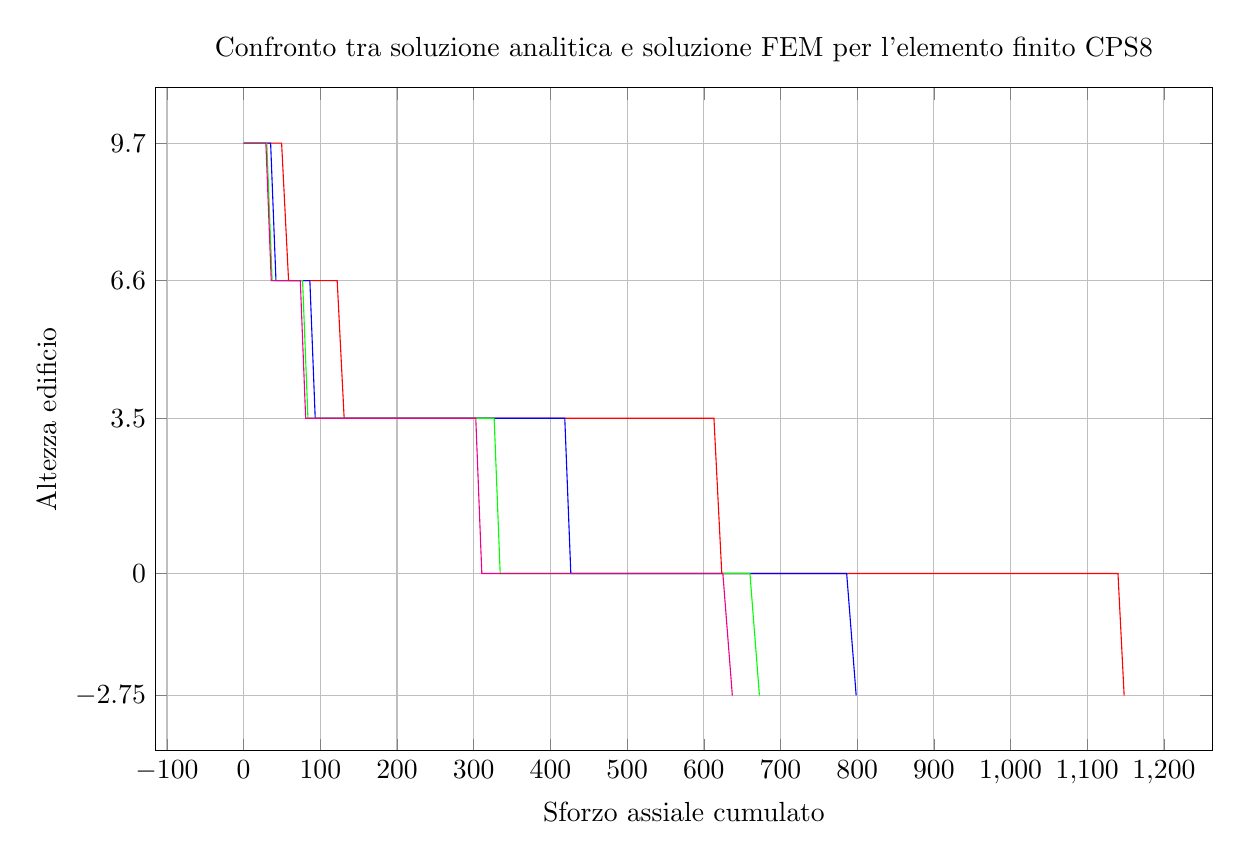
\begin{tikzpicture}\centering
	\begin{axis}[
	    height=10cm,
		width=15cm,
		grid=major,
		xlabel=Sforzo assiale cumulato,
		ylabel=Altezza edificio,
		ytick = {9.7,6.6,3.5,0,-2.75},
		title=Confronto tra soluzione analitica e soluzione FEM per l'elemento finito CPS8
    ]
	\addplot[color=red] coordinates {
	   (0000.00, 9.7  )
	   (0049.48, 9.7  )
	   (0058.55, 6.6  )
	   (0121.96, 6.6  )
	   (0131.03, 3.5  )
	   (0613.22, 3.5  )
	   (0623.45, 0    )
	   (1140.07, 0    )
	   (1148.11, -2.75)
	};
	\addplot[color=blue] coordinates {
	   (0000.00,  9.7  )
	   (0035.15, 9.7  )
	   (0042.12, 6.6  )
	   (0086.32, 6.6  )
	   (0093.29, 3.5  )
	   (0418.72, 3.5  )
	   (0426.59, 0    )
	   (0786.30, 0    )
	   (0798.68, -2.75)
	};
	\addplot[color=green] coordinates {
	   (0000.00,  9.7  )
	   (0030.15, 9.7  )
	   (0037.13, 6.6  )
	   (0076.82, 6.6  )
	   (0083.80, 3.5  )
	   (0326.63, 3.5  )
	   (0334.50, 0    )
	   (0660.16, 0    )
	   (0672.54, -2.75)
	};
	\addplot[color=magenta] coordinates {
	   (0000.00,  9.7  )
	   (0028.98, 9.7  )
	   (0035.96, 6.6  )
	   (0073.85, 6.6  )
	   (0080.83, 3.5  )
	   (0302.66, 3.5  )
	   (0310.53, 0    )
	   (0624.84, 0    )
	   (0637.22, -2.75)
	};
	\end{axis}
\end{tikzpicture}
